% Provenance (never printed): see sources/outline_sources.md (Year 1:
% observational astronomy, photometry). Telescopes, angular resolution,
% gratings, the Doppler effect and the black-body laws are owned by the
% physics series and recalled here. Curves computed in
% figdata/bachelor-1/{blackbody_bands, extinction_line}.py; numbers of the
% exercises and problem in the Book 3 scratch calculator ch02.py.
\chapter{التلسكوبات والكواشف والقياس الضوئي}\label{ch:b1:observing-the-sky}

ما تعرفه علوم الفلك عن النجوم، باستثناء بعض النيازك والعينات التي أُعيدت من القمر ومن الكويكبات، إنما تعلّمه من الضوء الذي ترسله. وهذا الضوء يعبر الغلاف الجوي للأرض، فيمتص مجالات كاملة من الأطوال الموجية ويطمس الباقي؛ ثم تجمعه مرآة يحدّ حجمها مدى خفوت التفاصيل التي يمكن رؤيتها ودقّتها؛ ثم يعدّه كاشف يحوّل الفوتونات إلى إلكترونات، وكل عدّ يحمل عدم يقين إحصائيًا. وقبل أن يتحوّل السطوع المقيس إلى \omterm{def:b1:observing-the-sky:flux}{إشعاعية} أو إلى مسافة، يجب أن تُفهم كل خطوة من هذه الخطوات وتُصحَّح. يتتبّع هذا الفصل الضوء من النجم إلى العدد: نوافذ الغلاف الجوي وقانون الإخماد، ثم التلسكوب \omterm{def:b1:observing-the-sky:seeing}{والرؤية الفلكية}، ثم الكاشف وضجيجه، ثم الأقدار والاختلاف المنظري والألوان التي تحوّل الدفوق المقيسة إلى خصائص للنجوم. والغلاف الجوي نفسه، إذا نُظر إليه من الأسفل، موضوع الفصول المناخية (\cref{ch:b1:radiation-heat-transport})؛ والقياس الضوئي نفسه، إذا طُبّق على الكواكب، يفتح الفصل التالي (\cref{ch:b1:comparative-planetology}).

\begin{recall}
يجمع الشيء المجمِّع للتلسكوب (العدسة أو المرآة الرئيسية) الضوءَ عبر فتحته، ويكوّن صورة في بؤرته؛ والحيود عبر فتحة قطرها $D$ يحدّ أصغر زاوية يفصلها بنحو $1.22\,\lambda/D$، وهو معيار رايلي (كتب الفيزياء للسنة الأولى). والمحزوز يفرّق الضوء بحسب الطول الموجي (كتب الفيزياء للسنة الثانية)، والمصدر المتحرك على خط النظر يزيح خطوطه الطيفية بتأثير دوبلر (الصف 12). والجسم في توازن حراري يصدر الطيف الجسمي الأسود، وتتبع ذروته قانون فين (كتب الفيزياء للسنة الثانية). وفي الكيمياء يتناسب امتصاص المحلول مع طول المسار.
\end{recall}

\section{نوافذ الغلاف الجوي}

الغلاف الجوي شفاف لبعض الأطوال الموجية، وغير شفاف لغيرها. وتمتص الإشعاعات أساسًا بخار الماء وثاني أكسيد الكربون والأوزون، وعند أقصر الأطوال الموجية تمتصها الذرات والجزيئات في الغلاف الجوي العلوي نفسه.
% ledger: nasa:ems-absorbers

\begin{definition}[النافذة الجوية]\label{def:b1:observing-the-sky:window}
\emph{النافذة الجوية}\index{النافذة الجوية} نطاق من الأطوال الموجية ينفذ فيه الغلاف الجوي معظم الإشعاع الذي يبلغ أعلاه ويصل إلى الأرض. وتمتد \emph{النافذة البصرية} من فوق البنفسجي القريب إلى تحت الأحمر القريب؛ أما \emph{نافذة الراديو} فمن أطوال موجية نحو سنتيمتر واحد إلى نحو عشرة أمتار.
\end{definition}

يعرض الشكل أدناه عتامة الغلاف الجوي من أشعة غاما إلى موجات الراديو الطويلة. فأشعة غاما والأشعة السينية وفوق البنفسجي دون نحو \qty{0.3}{\micro\metre} لا تبلغ الأرض أبدًا، ولذلك تُرصد من الفضاء. والضوء المرئي ينفذ، مع بعض الطمس. ومعظم تحت الحمراء يمتصه بخار الماء وثاني أكسيد الكربون، إلا في نوافذ ضيقة تستغلها المراصد الأرضية المرتفعة الجافة؛ وفيها تقع النطاقات الضوئية القريبة من تحت الحمراء، عند \qty{1.24}{\micro\metre} و\qty{1.65}{\micro\metre} و\qty{2.16}{\micro\metre}. وتُحجَب الأطوال الموجية من نحو \qty{30}{\micro\metre} حتى المليمتر من جديد؛ وتنفذ موجات الراديو من بضعة سنتيمترات إلى نحو عشرة أمتار، حتى من خلال الغيوم؛ أما الأطول فتعكسها طبقة الغلاف الأيوني.
% ledger: nasa:opacity-windows, baldry:2mass-pivot

\begin{omfigure}
\begin{tikzpicture}[x=1.0cm, y=2.2cm, font=\scriptsize]
% x = log10(lambda / 1 m) + 10 ; opacity 0..1 (schematic, after the NASA figure)
\fill[omSea!20] (0,0) rectangle (13,1.05);
\fill[brown!50] (0,0) -- (0,1) -- (3.45,1) -- (3.52,0.05) -- (4.03,0.05)
  -- (4.06,0.6) -- (4.09,0.15) -- (4.15,0.6) -- (4.22,0.15) -- (4.28,0.6)
  -- (4.34,0.15) -- (4.42,0.7) -- (4.55,0.25) -- (4.65,0.8) -- (4.9,0.2)
  -- (5.12,0.2) -- (5.25,0.7) -- (5.4,1) -- (7.0,1) -- (7.3,0.6) -- (7.6,0.75)
  -- (8.0,0.5) -- (8.5,0.03) -- (11.0,0.03) -- (11.3,1) -- (13,1) -- (13,0)
  -- cycle;
\draw[black!70] (0,0) rectangle (13,1.05);
\foreach \x in {0,...,13} { \draw (\x,0) -- (\x,-0.05); }
\foreach \x/\l in {0/0.1 nm, 2/10 nm, 4/1 \unit{\micro m}, 6/100 \unit{\micro m}, 8/1 cm,
  10/1 m, 12/100 m}
  { \node[below] at (\x,-0.05) {\l}; }
\foreach \y/\l in {0/0, 0.5/50, 1/100}
  { \draw (0,\y) -- (-0.1,\y); \node[left] at (-0.1,\y) {\l}; }
\node[rotate=90] at (-0.75,0.5) {\foreignlanguage{arabic}{العتامة \babelsublr{(\%)}}};
\node at (6.5,-0.42) {\small \foreignlanguage{arabic}{الطول الموجي، على مقياس لوغاريتمي}};
\node[align=center] at (1.7,0.75) {أشعة غاما، والأشعة السينية،\\ فوق البنفسجي};
\node[align=center] at (6.2,0.75) {تحت الحمراء\\ البعيدة};
\node[align=center] at (9.75,0.5) {نافذة الراديو};
\node[omThm] at (4.15,0.86) {J H K};
\draw[-{Stealth}] (2.6,1.25) node[above] {النافذة البصرية} -- (3.75,1.07);
\draw[-{Stealth}] (5.9,1.25) node[above] {نوافذ تحت الحمراء} -- (4.6,1.07);
\end{tikzpicture}

{\small عتامة الغلاف الجوي للإشعاع القادم من الفضاء، من \qty{0.1}{nm} إلى \qty{1}{km} (مقياس لوغاريتمي). الشكل تخطيطي، مأخوذ عن شكل لناسا في الملك العام: لا يهمّ هنا إلا النوافذ، لا الشكل الدقيق لكل نطاق امتصاص. تدلّ الحروف J وH وK على النطاقات الضوئية القريبة من تحت الأحمر.}
% ledger: nasa:opacity-windows, nasa:ems-absorbers, baldry:2mass-pivot
\end{omfigure}

\subsection*{الإخماد}

وحتى داخل النافذة البصرية يُزيل الغلاف الجوي جزءًا من الضوء، بالامتصاص وبالتشتت عن الجزيئات والهباء الجوي. وتُزيل طبقة رقيقة سمكها $\mathrm ds$ على طول الشعاع جزءًا من الشدة يتناسب مع $\mathrm ds$: $\mathrm dI = -\kappa I\,\mathrm ds$، حيث يتوقف معامل الإخماد $\kappa$ (لكل متر) على الطول الموجي وعلى تركيب الهواء عند ذلك الارتفاع. وهذا هو قانون امتصاص المحلول، مطبّقًا على عمود من الهواء.

\begin{proposition}[قانون بوغيه]\label{prop:b1:observing-the-sky:bouguer}
على شعاع يعبر وسطًا ممتصًّا تتناقص الشدة كما يلي
\[
  I = I_0\,e^{-\tau}, \qquad \tau = \int_0^s \kappa\,\mathrm ds' ,
\]
حيث $I_0$ الشدة الداخلة إلى الوسط، و$\tau$، العمق البصري للمسار، عدد لا بُعد له.
بالنسبة إلى غلاف جوي متوازي المستويات، يُرى نجم على البعد الزاوي $z$ عن \omterm{def:b1:spherical-astronomy:celestial-sphere}{سمت الرأس} (الزاوية بين اتجاهه والشاقول) عبر العمق البصري $\tau(z) = \tau_0\sec z$، حيث $\tau_0$ هو العمق البصري عند \omterm{def:b1:spherical-astronomy:celestial-sphere}{سمت الرأس}.
\end{proposition}

\begin{proof}
تنفصل المعادلة $\mathrm dI/I = -\kappa\,\mathrm ds$، ويُكامَل من أعلى الغلاف الجوي ($I = I_0$، $s = 0$) حتى الراصد، فيكون
$\ln(I/I_0) = -\int_0^s\kappa\,\mathrm ds'$. وفي غلاف جوي متوازي المستويات
يتعلّق $\kappa$ بالارتفاع $y$ وحده، ويقطع شعاعٌ مائل بالزاوية $z$ على الشاقول مسافة $\mathrm ds = \mathrm dy/\cos z$ ليصعد $\mathrm dy$. ومن ثَمّ
$\tau(z) = \int \kappa(y)\,\mathrm dy/\cos z = \tau_0\sec z$.
\end{proof}

\begin{definition}[الكتلة الهوائية، ومعامل الإخماد الجوي]\label{def:b1:observing-the-sky:extinction}
\emph{الكتلة الهوائية}\index{الكتلة الهوائية} $X$ لرصدٍ هي العمق البصري لخط النظر مقسومًا على العمق البصري عند \omterm{def:b1:spherical-astronomy:celestial-sphere}{سمت الرأس}: $X = \tau(z)/\tau_0$. وتساوي 1 عند \omterm{def:b1:spherical-astronomy:celestial-sphere}{سمت الرأس}، وفي غلاف متوازي المستويات $X = \sec z$. و\emph{معامل الإخماد الجوي}\index{معامل الإخماد الجوي} $k$ في نطاق معيّن هو مقدار الخفوت، بالقدر، الذي تُحدثه كتلة هوائية واحدة، فيُرصد نجم قدره $m_0$ فوق الغلاف الجوي عند
\[
  m = m_0 + kX .
\]
\end{definition}

يُعرَّف القدر في \cref{sec:b1:observing-the-sky:magnitudes}؛ ويكفي هنا أن نعلم أن الخفوت بعامل $e^{-\tau}$ يضيف $2.5\log_{10}e\;\tau = 1.086\,\tau$ قدرًا، إذن $k = 1.086\,\tau_0$. \omterm{def:b1:observing-the-sky:extinction}{والكتلة الهوائية} للغلاف المتوازي المستويات دقيقة جدًا حتى ارتفاع نحو \ang{30} ($X = 2$)، وتفشل قرب الأفق، حيث يتزايد $\sec z$ دون حدّ بينما يبقى المسار الحقيقي عبر غلاف منحنٍ منتهيًا؛ ولهذا يتجنّب الراصدون الارتفاعات المنخفضة، وكذلك بسبب الطمس الذي يزداد مع طول المسار.

\begin{method}[خط الإخماد]\label{met:b1:observing-the-sky:extinction-line}
لإيجاد القدر $m_0$ الذي يكون للنجم فوق الغلاف الجوي:
\begin{enumerate}
  \item قِس القدر $m$ للنجم، أو لنجم معياري، عند عدة كتل هوائية خلال الليل، أثناء طلوعه أو غروبه؛
  \item احسب كل كتلة هوائية من البعد عن \omterm{def:b1:spherical-astronomy:celestial-sphere}{سمت الرأس}، $X = \sec z$؛
  \item ارسم $m$ بدلالة $X$، وأجرِ مطابقةً بخط مستقيم بطريقة المربعات الصغرى؛
  \item الميل هو معامل الإخماد $k$ لتلك الليلة في ذلك النطاق؛ والقطعة عند $X = 0$ هي $m_0$.
\end{enumerate}
ويُصحّح المعامل $k$ نفسه بعد ذلك كل نجم آخر رُصد في تلك الليلة وفي النطاق نفسه: $m_0 = m - kX$.
\end{method}

\begin{example}
في ليلة واحدة قِيس نجم ست مرات في النطاق V:
\begin{center}
\small
\begin{tabular}{lcccccc}
\hline
$X$ & 1.05 & 1.18 & 1.36 & 1.62 & 1.95 & 2.31 \\
$m$ & 8.024 & 8.031 & 8.072 & 8.104 & 8.171 & 8.216 \\
\hline
\end{tabular}
\end{center}
يمرّ خط المربعات الصغرى، المرسوم في الشكل أدناه، بميل $k = \qty{0.160}{\mag}$ لكل كتلة هوائية، وبقطعة $m_0 = 7.851$. وتتشتت النقاط حوله بمقدار \num{0.006} قدرًا، وهي دقة ليلة قياس ضوئي جيدة. وعند \omterm{def:b1:spherical-astronomy:celestial-sphere}{سمت الرأس} يُخفت النجم بمقدار \num{0.16} قدرًا، أي خسارة $1 - 10^{-0.4\times0.160} = \qty{14}{\percent}$ من ضوئه.
\end{example}

\begin{omfigure}
\begin{tikzpicture}
\begin{axis}[omrecord, width=0.62\linewidth, height=5.4cm, xmin=0, xmax=2.5,
  ymin=7.80, ymax=8.28, y dir=reverse, xlabel={\foreignlanguage{arabic}{الكتلة الهوائية $X$}},
  ylabel={\foreignlanguage{arabic}{القدر $m$}}, yticklabel style={/pgf/number format/fixed,
  /pgf/number format/precision=2}, tick label style={font=\scriptsize},
  label style={font=\small}]
\addplot[omThm, line width=0.9pt, dashed] table[x=X, y=m] {figdata/out/bachelor-1-extinction_line-fit.dat};
\addplot[only marks, mark=*, mark size=1.6pt, omDef] table[x=X, y=m] {figdata/out/bachelor-1-extinction_line-obs.dat};
\node[font=\scriptsize, right, fill=white, inner sep=1pt] at (axis cs:0.05,7.83) {$m_0 = 7.851$};
\node[font=\scriptsize, fill=white, inner sep=1pt, rotate=-10] at (axis cs:0.95,8.10) {الميل $k = 0.160$};
\end{axis}
\end{tikzpicture}

{\small خط إخماد: قدرُ نجم واحد عند ست كتل هوائية (النقاط)، وخط المربعات الصغرى ممدودًا حتى $X = 0$، أي القدر فوق الغلاف الجوي. وتزداد الأقدار نحو الأسفل: فالنجم الأخفت يقع أسفل.}
\end{omfigure}

\subsection*{الرؤية الفلكية}

لا يهدأ الهواء فوق التلسكوب أبدًا. فجيوب الهواء ذات الحرارات المختلفة قليلًا، وبالتالي معاملات الانكسار المختلفة قليلًا، تنجرف عبر الحزمة فتنحرفها بزوايا عشوائية صغيرة، وتتغيّر عشرات المرات في الثانية. فالعين ترى النجم يومض؛ والتعريض الطويل يسجّل بقعة مطموسة أكبر بكثير من نمط الحيود للتلسكوب.

\begin{definition}[الرؤية الفلكية]\label{def:b1:observing-the-sky:seeing}
\emph{الرؤية الفلكية}\index{الرؤية الفلكية} عند موقع هي القطر الزاوي لصورة منبع نقطي يطمسه اضطراب الغلاف الجوي في تعريض طويل، وتُقاس بالعرض الكامل عند نصف القيمة العظمى للصورة، بالثواني القوسية.
\end{definition}

تتغيّر \omterm{def:b1:observing-the-sky:seeing}{الرؤية الفلكية} من ليلة إلى أخرى ومن ساعة إلى أخرى، وتُختار المواقع لأجلها: فعلى قمة ماونا كيا، على ارتفاع \qty{4204}{m}، تبلغ الرؤية الوسيطة للغلاف الحر نحو \ang{;;0.40}، وتتراوح من نحو \ang{;;0.45} شتاءً إلى \ang{;;0.35} صيفًا، وتكون أفضل عُشر الليالي دون نحو \ang{;;0.25}؛ والموقع نفسه لا يحوي فوقه إلا \qty{0.9}{mm} من بخار الماء القابل للترسيب، وهذا ما يفتح نوافذه تحت الحمراء.
% ledger: cfht:site, cfht:seeing

\section{التلسكوبات وقدرة التفريق}

يؤدي التلسكوب أمرين: يجمع الضوء على مساحة عدسته أو مرآته الرئيسية، ويكوّن صورة تتميز فيها التفاصيل. والمساحة المجمِّعة تنمو تناسبًا مع $D^2$: فمرآة ضعف العرض تجمع أربعة أمثال الفوتونات في الزمن نفسه، وتبلغ نجومًا أخفت بأربع مرات. ويحدّ الحيود قدرةَ التفريق بنحو $1.22\,\lambda/D$، وتحدّها \omterm{def:b1:observing-the-sky:seeing}{الرؤية الفلكية} أيضًا.

\begin{example}
يبلغ قطر فتحة تلسكوب كندا–فرنسا–هاواي على ماونا كيا \qty{3.58}{m}. وعند \qty{550}{nm} يكون حدّه الحيودي
\[
  1.22\times\frac{\qty{550e-9}{m}}{\qty{3.58}{m}} = \qty{1.87e-7}{rad}
  = \ang{;;0.039},
\]
أدقّ بعشر مرات من \omterm{def:b1:observing-the-sky:seeing}{الرؤية الفلكية} الوسيطة البالغة \ang{;;0.40} في الموقع نفسه. ويتساوى الحدّان في مرآة قطرها $D = 1.22\lambda/\theta =
1.22\times\qty{550e-9}{m}/(\num{0.40}/\num{206265}) = \qty{0.35}{m}$: فكل تلسكوب أرضي أوسع من نحو \qty{35}{cm} تحدّه \omterm{def:b1:observing-the-sky:seeing}{الرؤية الفلكية}، لا بصرياته الذاتية، عند الأطوال الموجية المرئية.
% ledger: cfht:aperture, cfht:seeing
\end{example}

ولذلك لا يكسب التلسكوب الأرضي الكبير مساحة تجميع فحسب، لا حِدّةً، ما لم يُصحّح الاضطراب. و\emph{البصريات التكيفية} تفعل ذلك: فمجسّ يقيس، مرات عدة في الثانية، مقدار تشوّه الجبهة الموجية الآتية من نجم ساطع (أو من نجم صناعي يُصنع بليزر في الغلاف الجوي العلوي)، ومرآة رقيقة تنحني بمحرّكات صغيرة كثيرة تلغي التشوّه. ويعمل التصحيح أفضل ما يكون في تحت الحمراء، حيث يكون الاضطراب أبطأ وأضعف، وفي حقل صغير حول نجم الدليل. ولا توجد أيّ رؤية فلكية في الفضاء.

\section{الكواشف}

تُجمِّع العين الضوء لجزء من الثانية، وتستجيب لجزء صغير من الفوتونات الداخلة إليها. وكانت الألواح الفوتوغرافية تُجمِّع الضوء ساعات، لكنها تسجّل منه جزءًا صغيرًا فقط. ويستعمل علم الفلك الحديث كواشف فوتونية مصنوعة من أشباه الموصلات، يحرّر فيها كل فوتون ممتص ذو طاقة كافية إلكترونًا.

\begin{definition}[الكفاءة الكمومية، ونسبة الإشارة إلى الضجيج]\label{def:b1:observing-the-sky:detector}
\emph{الكفاءة الكمومية}\index{الكفاءة الكمومية} $\eta$ للكاشف عند طول موجي معيّن هي الكسر من الفوتونات الساقطة الذي يسجّله، على شكل إلكترونات ضوئية: $\eta = N_\mathrm{e}/N_\gamma$. و\emph{نسبة الإشارة إلى الضجيج}\index{نسبة الإشارة إلى الضجيج} لقياسٍ ما هي الإشارة المقيسة مقسومةً على انحرافها المعياري، أي الحجم المعتاد لخطئه العشوائي.
\end{definition}

\emph{الشحنة المقترنة} (CCD) هي الكاشف المعياري للنافذة البصرية. وهي شريحة رقيقة من السيليكون مقسّمة إلى شبكة من البكسلات، كل بكسل بئر جهد يخزّن الإلكترونات التي حرّرتها الفوتونات الممتصة فيه أثناء التعريض. وفي نهاية التعريض تُطبَّق على الأقطاب فولتيات بالتتابع، فتنقل الشحنات من بكسل إلى آخر، صفًّا صفًّا، إلى مكبّر واحد يقيسها واحدةً واحدة؛ والصورة هي جدول العدّ. ويسجّل الكاشف CCD نسبة كبيرة من الفوتونات الساقطة على معظم الطيف المرئي، وتتناسب استجابته مع الضوء الوارد حتى حدٍّ أقصى للشحنة في كل بكسل (\emph{سعة البئر الممتلئة})، ويمكنه أن يجمّع ساعات. وتعمل المصفوفات تحت الحمراء بالمبدأ نفسه، بأشباه موصلات أخرى، وتُقرأ بكسلًا بكسل.

تصل الفوتونات عشوائيًا. فإذا أرسل مصدر في المتوسط $N$ إلكترونًا ضوئيًا أثناء التعريض، فإن العدّ المسجَّل فعلًا يتذبذب من تعريض إلى آخر بانحراف معياري $\sqrt N$ (إحصاء بواسون، المقبول من نظرية الاحتمال: عدّ الأحداث النادرة المستقلة).

\begin{proposition}[ضجيج الفوتونات]\label{prop:b1:observing-the-sky:snr}
عندما يغلب ضجيج الفوتونات الصادر من المصدر وحده، يُقاس مصدر يعطي $R$ إلكترونًا ضوئيًا في الثانية في زمن $t$ بنسبة إشارة إلى ضجيج
\[
  \mathrm{SNR} = \frac{Rt}{\sqrt{Rt}} = \sqrt{Rt} ;
\]
تنمو كالجذر التربيعي لزمن التعريض، وكقطر التلسكوب (لأن $R \propto D^2$). والخطأ في القدر هو عندئذٍ $\sigma_m \approx 1.086/\mathrm{SNR}$.
\end{proposition}

\begin{proof}
الإشارة هي $N = Rt$ وانحرافها المعياري $\sqrt N$. وبالنسبة إلى القدر، $m = -2.5\log_{10}N + \text{ثابت}$، فيعطي خطأ صغير $\sigma_N$ الخطأ $\sigma_m = 2.5\log_{10}e\;\sigma_N/N = 1.086/\mathrm{SNR}$.
\end{proof}

لقياس قدر بدقة \num{0.01} تلزم نسبة إشارة إلى ضجيج نحو 109، أي نحو \num{12000} إلكترون ضوئي. وبالنسبة إلى المصادر الخافتة يدخل حدّان آخران: فالسماء نفسها تتوهّج، وكل بكسل من صورة النجم يجمع فوتونات السماء أيضًا، بمعدّل $B$؛ والمكبّر يضيف ضجيج قراءة $\sigma_r$ إلى كل بكسل يُقرأ. والعبارة الكاملة،
\[
  \mathrm{SNR} = \frac{Rt}{\sqrt{Rt + Bt + n\sigma_r^2}}
\]
على $n$ بكسل من الصورة، تُختزل إلى $\sqrt{Rt}$ لنجم ساطع، وإلى $R\sqrt t/\sqrt B$ لمصدر أخفت من السماء. ولأن $B$ يتزايد مع مساحة قرص \omterm{def:b1:observing-the-sky:seeing}{الرؤية الفلكية}، فإن الرؤية الجيدة تفيد مرتين: فالصورة الأحدّ تفرّق أكثر وتجمع سماءً أقل (\cref{exo:b1:observing-the-sky:11}).

\begin{inthefield}[ليلة عند التلسكوب]
يُجرى القياس الضوئي بالمعايرات بقدر ما يُجرى بالنجوم. فقبل الليلة يأخذ الراصد في مرصد احترافي إطارات \emph{الانحياز} (تعريضات بطول صفري تسجّل الإزاحة الكهربائية لكل بكسل)، و\emph{حقول التسوية} (صور للداخل المضاء بانتظام للقبة أو لسماء الشفق، تُظهر كيف تتفاوت الحساسية من بكسل إلى آخر وعبر الحقل)؛ وتُصحَّح صور الرصد بطرح الانحياز والقسمة على حقل التسوية. وخلال الليل تُرصد نجوم معيارية ذات أقدار معروفة عند عدة كتل هوائية لتحديد خط الإخماد ونقطة الصفر التي تحوّل العدّ إلى أقدار. وتُسمّى الليلة \emph{فوتومترية} حين يبقى الإخماد ثابتًا بما يكفي لصلاحية هذا التصحيح؛ وعلى قمة ماونا كيا تكون \qty{55}{\percent} من الليالي فوتومترية.
% ledger: cfht:nights
\begin{center}
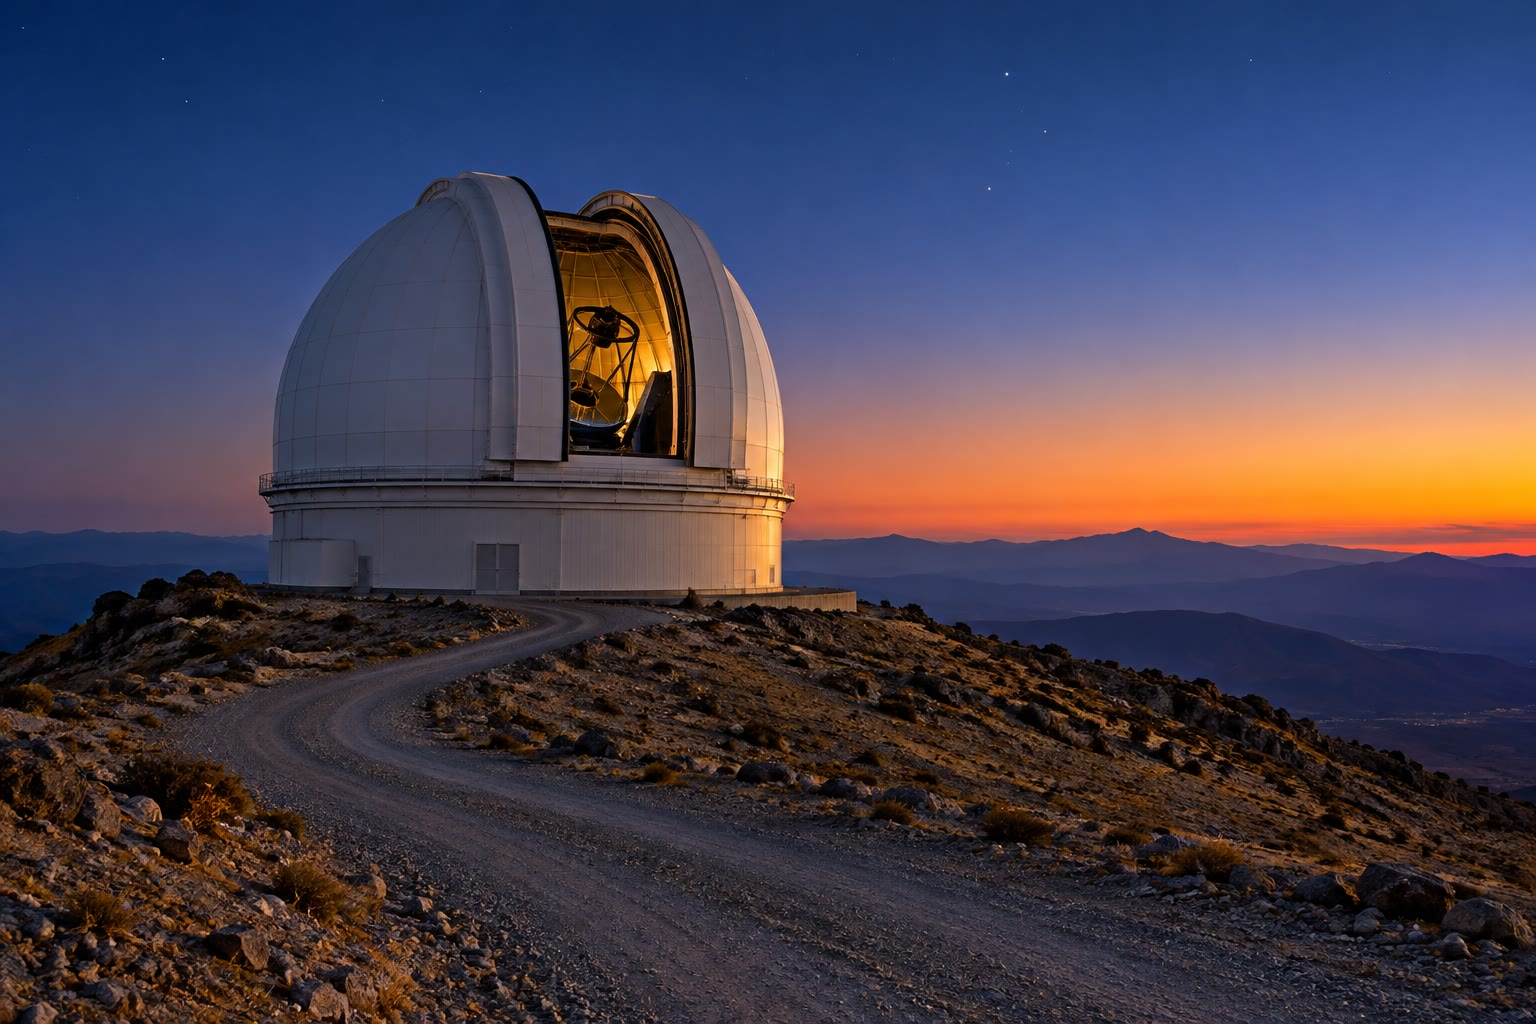
\includegraphics[width=0.55\linewidth]{images/book3/ai/b1-observatory-dusk.jpg}
\end{center}
\end{inthefield}

\section{الدفوق والأقدار}\label{sec:b1:observing-the-sky:magnitudes}

\begin{definition}[الدفق والإشعاعية]\label{def:b1:observing-the-sky:flux}
\emph{الدفق}\index{الدفق (لمصدر)} $F$ الذي يصل من مصدر هو قدرة إشعاعه العابرة لوحدة مساحة مُقامة عموديًا على اتجاهه، بالواط لكل متر مربع؛ وإذا قُصر على نطاق من الأطوال الموجية فهو الدفق في ذلك النطاق. و\emph{الإشعاعية}\index{الإشعاعية} $L$ للمصدر هي القدرة الكلية التي يشعّها، بالواط.
\end{definition}

\begin{proposition}[قانون التربيع العكسي]\label{prop:b1:observing-the-sky:inverse-square}
مصدر إشعاعيته $L$ يشعّ بالتساوي في كل الاتجاهات، يُرى على بعد $d$ عبر الفراغ، يعطي \omterm{def:b1:observing-the-sky:flux}{الدفق}
\[
  F = \frac{L}{4\pi d^2} .
\]
\end{proposition}

\begin{proof}
في حالة مستقرة بلا امتصاص تكون القدرة العابرة لأيّ كرة مركزها المصدر واحدة، أي $L$، بحفظ الطاقة. وبالتماثل تتوزّع بالتساوي على مساحة الكرة $4\pi d^2$.
\end{proof}

\begin{example}
\omterm{def:b1:observing-the-sky:flux}{إشعاعية} الشمس هي \qty{3.828e26}{W}. وعلى مسافة وحدة فلكية واحدة، \qty{1.496e11}{m}، يكون دفقها $\num{3.828e26}/(4\pi\times
(\num{1.496e11})^2) = \qty{1361}{W.m^{-2}}$: وهو الإشعاع الشمسي الذي تتلقاه الأرض عند أعلى غلافها الجوي.
% ledger: sun:L, const:au, earth:TSI
\end{example}

تمتد الدفوق على مدى هائل، ويقارن الفلكيون بينها على مقياس لوغاريتمي موروث من الفئات التي صُنّفت فيها النجوم المرئية بالعين قديمًا، من الأسطع في القدر الأول إلى الأخفت في القدر السادس.

\begin{definition}[القدر الظاهري، والنطاق الضوئي]\label{def:b1:observing-the-sky:magnitude}
\emph{النطاق الضوئي}\index{النطاق الضوئي} نطاق من الأطوال الموجية يحدّده مرشّح معياري، ويُسمّى بحرف: U (فوق البنفسجي)، وB (أزرق)، وV (مرئي)، وR (أحمر)، وI (تحت أحمر قريب)، وJ وH وK في النوافذ تحت الحمراء. و\emph{القدر الظاهري}\index{القدر الظاهري} $m$ لمصدر في نطاق يُعرَّف بدلالة دفقه $F$ في ذلك النطاق بالعلاقة
\[
  m_1 - m_2 = -2.5\log_{10}\frac{F_1}{F_2} ,
\]
ويُحدَّد نقطة الصفر بالنجوم المعيارية، وهي قريبة من قدر النجم فيغا في كل نطاق. والفرق قدره 5 أقدار يعادل عاملًا قدره 100 بالضبط في \omterm{def:b1:observing-the-sky:flux}{الدفق}؛ والقدر الواحد عامل $100^{1/5} = 2.512$. وتكون المصادر الأسطع أصغر أقدارًا، وربما سالبة.
\end{definition}

أطوال الموجات المركزية للمرشّحات المعيارية U وB وV وR وI هي
\qty{358.5}{nm}، \qty{437.1}{nm}، \qty{547.8}{nm}، \qty{650.4}{nm} و\qty{802.0}{nm}.
% ledger: baldry:bessell-pivot
ففي النطاق V، للشمس \omterm{def:b1:observing-the-sky:magnitude}{القدر الظاهري} $-26.74$، ولسيريوس، ألمع نجوم السماء الليلية، $-1.46$، ولفيغا $0.03$. فالشمس إذن أسطع من سيريوس في سمائنا بمقدار $10^{0.4\times(26.74 - 1.46)} = \num{1.29e10}$ مرة؛ وهذا لا يخبرنا بعدُ أيّهما يشعّ أكثر، فذلك يتطلب المسافات.
% ledger: nasa:sun-V, simbad:sirius, simbad:vega

\subsection*{الاختلاف المنظري والفرسخ الفلكي}

وبدوران الأرض حول الشمس يبدو النجم القريب كأنه يتحرك على خلفية النجوم الأبعد بكثير، فيرسم في السنة قطعًا ناقصًا صغيرًا. وهذه الحركة الظاهرة هي أكثر القياسات مباشرةً لمسافات النجوم: إذ تستعمل مدار الأرض خطَّ أساس للمساح.

\begin{definition}[الاختلاف المنظري السنوي، والفرسخ الفلكي]\label{def:b1:observing-the-sky:parallax}
\emph{الاختلاف المنظري السنوي}\index{الاختلاف المنظري السنوي} $p$ لنجم هو الزاوية التي يحصرها عند النجم نصف قطر مدار الأرض، أي وحدة فلكية واحدة، مرئيًا عموديًا على خط النظر؛ وهو نصف المحور الأكبر للقطع الناقص السنوي الذي يبدو أن النجم يرسمه. و
\emph{الفرسخ الفلكي}\index{الفرسخ الفلكي} (\unit{\parsec}) هو البعد الذي تحصر عنده الوحدة الفلكية ثانيةً قوسيةً واحدة:
\[
  \qty{1}{\parsec} = \frac{\qty{1}{\au}}{\tan\ang{;;1}} = \qty{206265}{\au}
  = \qty{3.0857e16}{m} = \qty{3.2616}{\lightyear} .
\]
\end{definition}

ولأن $p$ صغير، يكون $\tan p \approx p$ بالراديان، ويتبع البعد فورًا:
\[
  d = \frac{\qty{1}{\au}}{\tan p} \quad\Longrightarrow\quad
  \frac{d}{\unit{\parsec}} = \frac{1}{p/\text{ثانية قوسية}} .
\]
ويبلغ اختلاف سيريوس المنظري \ang{;;0.37921}، فيقع على بعد $1/0.37921 =
\qty{2.637}{\parsec}$، أي \qty{8.60}{\lightyear}. وحتى أقرب النجوم لا يتجاوز اختلافها المنظري ثانيةً قوسيةً واحدة، وهو أصغر من \omterm{def:b1:observing-the-sky:seeing}{الرؤية الفلكية}: ويُستخلص الاختلاف المنظري من إزاحة مركز صورة النجم، وهذا المركز تحدّده فوتونات كثيرة بدقة تفوق كثيرًا عرض الصورة. وقد قاست بعثة فضائية موصوفة في نهاية هذا الفصل مواضع نحو مليارين من الأجرام بهذه الطريقة.
% ledger: simbad:sirius, const:au, esa:gaia

\begin{omfigure}
\begin{tikzpicture}[font=\small]
\draw[black!50] (0,0) ellipse (2.0cm and 0.55cm);
\fill[orange!80!black] (0,0) circle (3pt) node[below=3pt] {الشمس};
\fill[blue!70!black] (-2.0,0) circle (2pt) node[left, align=right] {الأرض، بعد ستة\\ أشهر};
\fill[blue!70!black] (2.0,0) circle (2pt) node[right] {الأرض};
\fill (0,4.4) circle (1.6pt) node[above] {النجم};
\draw[omDef, thick] (0,0) -- node[right, pos=0.55] {$d$} (0,4.4);
\draw[omThm] (2.0,0) -- (0,4.4);
\draw[omThm, dashed] (-2.0,0) -- (0,4.4);
\draw[thick] (0,0) -- node[above] {\qty{1}{\au}} (2.0,0);
\draw[omThm] (0,3.75) arc[start angle=-90, end angle=-65.6, radius=0.65cm];
\node[omThm] at (0.17,3.38) {$p$};
\end{tikzpicture}

{\small \omterm{def:b1:observing-the-sky:parallax}{الاختلاف المنظري السنوي} (غير مرسوم بمقياس): يُرى من النجم، فيحصر نصف مدار الأرض الزاوية $p$. وعلى بُعد ستة أشهر يختلف اتجاه النجم بمقدار $2p$. والزاوية الحقيقية لأقرب النجوم أقل من ثانية قوسية واحدة.}
\end{omfigure}

\begin{definition}[القدر المطلق، ومعامل المسافة]\label{def:b1:observing-the-sky:absolute}
\emph{القدر المطلق}\index{القدر المطلق} $M$ لنجم في نطاق هو \omterm{def:b1:observing-the-sky:magnitude}{القدر الظاهري} الذي كان سيكون له على بعد \qty{10}{\parsec}، مرئيًا عبر الفراغ. والفرق $m - M$ هو \emph{معامل المسافة}\index{معامل المسافة}.
\end{definition}

\begin{proposition}[معامل المسافة]\label{prop:b1:observing-the-sky:modulus}
لنجم على بُعد $d$ مرئيًّا عبر الفراغ،
\[
  m - M = 5\log_{10}\frac{d}{\qty{10}{\parsec}} .
\]
إذا خفّ الضوء في طريقه بمقدار $A$ من القدر بسبب الإخماد، فإن $m - M = 5\log_{10}(d/\qty{10}{\parsec}) + A$. وفي نطاق واحد تكون نسبة إشعاعيتي نجمين $L_1/L_2 = 10^{0.4(M_2 - M_1)}$.
\end{proposition}

\begin{proof}
بقانون التربيع العكسي يكون \omterm{def:b1:observing-the-sky:flux}{الدفق} عند $d$ \omterm{def:b1:observing-the-sky:flux}{والدفق} عند \qty{10}{\parsec} بنسبة $F(d)/F(\qty{10}{\parsec}) = (\qty{10}{\parsec}/d)^2$. وتعريف الأقدار يعطي $m - M = -2.5\log_{10}(\qty{10}{\parsec}/d)^2
= 5\log_{10}(d/\qty{10}{\parsec})$. ويضرب الإخماد \omterm{def:b1:observing-the-sky:flux}{الدفق} في $10^{-0.4A}$، فيضيف $A$ إلى $m$. وعند البعد المشترك \qty{10}{\parsec} تكون الدفوق بنسبة \omterm{def:b1:observing-the-sky:flux}{الإشعاعيات}، و$M_1 - M_2 = -2.5\log_{10}(L_1/L_2)$.
\end{proof}

للشمس \omterm{def:b1:observing-the-sky:absolute}{القدر المطلق} $M_\odot = 4.83$ \omterm{def:b1:observing-the-sky:flux}{والإشعاعية} \qty{3.828e26}{W}. ومقارنة \omterm{def:b1:observing-the-sky:absolute}{القدر المطلق} لنجم في النطاق V بقدر الشمس تعطي إشعاعيته في V بالوحدات الشمسية، $L/L_\odot = 10^{0.4(4.83 - M)}$ --- وهي \omterm{def:b1:observing-the-sky:flux}{إشعاعية} \emph{النطاق V}، لأن نجمًا أحرّ بكثير من الشمس أو أبرد يضع جزءًا مختلفًا من قدرته خارج النطاق V.
% ledger: sun:Mabs, sun:L

\subsection*{اللون}

\begin{definition}[دليل اللون]\label{def:b1:observing-the-sky:colour-index}
\emph{دليل اللون}\index{دليل اللون} لنجم هو فرق قدريه في نطاقين، يُكتب الأزرق منهما أولًا؛ وأشهره $B - V$. فالقيمة الصغيرة أو السالبة للمقدار $B - V$ تميّز نجمًا أزرق، والكبيرة نجمًا أحمر.
\end{definition}

\omterm{def:b1:observing-the-sky:colour-index}{ودليل اللون} لا يتعلّق بالبعد، لأن قانون التربيع العكسي يُخفت النطاقين بالقدر نفسه؛ وهو يقيس شكل الطيف، ومن ثَمّ درجة حرارة سطح النجم. والنجم يشعّ تقريبًا كجسم أسود تبلغ ذروة طيفه عند $\lambda_\mathrm{max} = b/T$ (قانون فين، بثابت $b = \qty{2.898e-3}{m.K}$، وهو مقبول من كتاب الفيزياء للسنة الثانية).
يرسم الشكل أدناه ثلاثة أطياف للجسم الأسود: جسم بارد عند \qty{3500}{K} تبلغ ذروته في تحت الحمراء القريب، ويعطي دفقًا أكبر في V منه في B؛ والحرارة الفعّالة للشمس، \qty{5772}{K}، تضع ذروتها عند \qty{502}{nm}، بين B وV؛ وجسم عند \qty{10000}{K} تبلغ ذروته في فوق البنفسجي ويكون أسطع في B منه في V. وتزداد نسبة شدّتي B وV باطّراد مع الحرارة، من \num{0.46} إلى \num{0.97} ثم \num{1.53} للمنحنيات الثلاثة، ولهذا يتناقص $B - V$ كلما ارتفعت $T$.
% ledger: const:b, nasa:sun-Teff, baldry:bessell-pivot

\begin{omfigure}
\begin{tikzpicture}
\begin{axis}[omrecord, width=0.9\linewidth, height=5.8cm, xmin=200, xmax=1500,
  ymin=0, ymax=1.17, xtick={200,400,...,1400}, ytick={0,0.5,1},
  xlabel={\foreignlanguage{arabic}{الطول الموجي \babelsublr{(\unit{nm})}}},
  ylabel={\foreignlanguage{arabic}{$B_\lambda$ على القيمة العظمى}}, tick label style={font=\scriptsize},
  label style={font=\small}, legend style={font=\scriptsize, at={(0.5,1.03)},
  anchor=south, draw=none, fill=none}, legend columns=3]
\addplot[red!75!black, line width=1.1pt] table[x=lam_nm, y=t3500] {figdata/out/bachelor-1-blackbody_bands-curves.dat};
\addplot[orange!90!black, line width=1.1pt] table[x=lam_nm, y=t5772] {figdata/out/bachelor-1-blackbody_bands-curves.dat};
\addplot[omDef, line width=1.1pt] table[x=lam_nm, y=t10000] {figdata/out/bachelor-1-blackbody_bands-curves.dat};
\legend{{\mbox{\textdir TLT \qty{3500}{K}}}, {\mbox{\textdir TLT \qty{5772}{K}} للشمس}, {\mbox{\textdir TLT \qty{10000}{K}}}}
\draw[black!45, densely dashed] (axis cs:358.5,0) -- (axis cs:358.5,1.06);
\node[font=\scriptsize, above, inner sep=1pt] at (axis cs:358.5,1.06) {U};
\draw[black!45, densely dashed] (axis cs:437.1,0) -- (axis cs:437.1,1.06);
\node[font=\scriptsize, above, inner sep=1pt] at (axis cs:437.1,1.06) {B};
\draw[black!45, densely dashed] (axis cs:547.8,0) -- (axis cs:547.8,1.06);
\node[font=\scriptsize, above, inner sep=1pt] at (axis cs:547.8,1.06) {V};
\draw[black!45, densely dashed] (axis cs:650.4,0) -- (axis cs:650.4,1.06);
\node[font=\scriptsize, above, inner sep=1pt] at (axis cs:650.4,1.06) {R};
\draw[black!45, densely dashed] (axis cs:802.0,0) -- (axis cs:802.0,1.06);
\node[font=\scriptsize, above, inner sep=1pt] at (axis cs:802.0,1.06) {I};
\end{axis}
\end{tikzpicture}

{\small أطياف الجسم الأسود عند ثلاث حرارات، مقسومةً كل منها على قيمتها العظمى، مع الأطوال الموجية المحورية لمرشّحات U وB وV وR وI (منقّطة). وتنتقل الذروة نحو الأطوال الأقصر كلما ارتفعت الحرارة (قانون فين): \qty{828}{nm} و\qty{502}{nm} و\qty{290}{nm}.}
% ledger: const:h, const:c, const:kB, const:b, nasa:sun-Teff, baldry:bessell-pivot
\end{omfigure}

تُظهر أربعة نجوم ساطعة مدى الألوان:
\begin{center}
\small
\begin{tabular}{lcccc}
\hline
النجم & $V$ & $B$ & $B - V$ & الاختلاف المنظري \babelsublr{(\unit{mas})} \\
\hline
ريجل & \mbox{\textdir TLT 0.13} & \mbox{\textdir TLT 0.10} & $-0.03$ & \mbox{\textdir TLT 3.78} \\
ألتير & \mbox{\textdir TLT 0.76} & \mbox{\textdir TLT 0.98} & \mbox{\textdir TLT 0.22} & \mbox{\textdir TLT 194.95} \\
بولاريس & \mbox{\textdir TLT 2.02} & \mbox{\textdir TLT 2.62} & \mbox{\textdir TLT 0.60} & \mbox{\textdir TLT 7.54} \\
بيتلجوز & \mbox{\textdir TLT 0.42} & \mbox{\textdir TLT 2.27} & \mbox{\textdir TLT 1.85} & \mbox{\textdir TLT 6.55} \\
\hline
\end{tabular}
\end{center}
% ledger: simbad:rigel, simbad:altair, simbad:polaris, simbad:betelgeuse
ريجل أبيض مزرقّ، وبيتلجوز في الكوكبة نفسها برتقالي محمرّ: فرق في اللون يُرى بالعين المجردة. وأنواعهما الطيفية، B8 وM1--M2، تقول الشيء نفسه بلغة الأطياف، وهي موضوع الكتاب 5.

\section{المطيافات}

يقيس القياس الضوئي الضوء في نطاقات عريضة قليلة، أما المطياف فيبسطه طيفًا. ويعبر الضوء من بؤرة التلسكوب شقًّا ضيقًا، ويُجعَل متوازيًا بمُسوٍّ، ويُفرَّق بمحزوز (أو بمنشور)، ثم تركّزه آلة تصوير على كاشف، فيقع كل طول موجي على عمود مختلف من البكسلات (انظر الشكل أدناه). ومحزوز عدد خطوطه المضاءة $N$، يُستعمل في الرتبة $k$، يفصل طولين موجيين تفصل بينهما $\Delta\lambda$ إذا كان $\lambda/\Delta\lambda \le kN$، وهذه قدرته على التفريق (مذكورة من كتاب الفيزياء للسنة الثانية).

\begin{omfigure}
\begin{tikzpicture}[font=\scriptsize, >=Stealth]
\draw[thick, fill=omSea!25] (0.15,0) ellipse (0.13 and 0.9);
\node[below] at (0.15,-0.95) {المُجمِّعة};
\draw[omDef] (-1.3,0.75) -- (0.15,0.75) -- (2.4,0);
\draw[omDef] (-1.3,-0.75) -- (0.15,-0.75) -- (2.4,0);
\draw[omDef, ->] (-1.3,0) -- (-0.2,0);
\node[above] at (-0.8,0.75) {ضوء النجم};
\draw[very thick] (2.4,-0.35) -- (2.4,-0.06); \draw[very thick] (2.4,0.06) -- (2.4,0.35);
\node[above] at (2.4,0.38) {الشق};
\draw[omDef] (2.4,0) -- (3.6,0.55); \draw[omDef] (2.4,0) -- (3.6,-0.55);
\draw[thick, fill=omSea!25] (3.6,0) ellipse (0.1 and 0.72);
\node[below] at (3.6,-0.74) {المسوِّي};
\draw[omDef] (3.6,0.55) -- (4.9,0.55); \draw[omDef] (3.6,-0.55) -- (4.9,-0.55);
\draw[thick, pattern=north east lines] (4.85,-0.8) rectangle (5.0,0.8);
\node[below] at (4.92,-0.82) {المحزوز};
\draw[blue!70!black] (5.0,0.3) -- (6.4,0.95); \draw[red!70!black] (5.0,0.3) -- (6.4,-0.15);
\draw[blue!70!black] (5.0,-0.3) -- (6.4,0.35); \draw[red!70!black] (5.0,-0.3) -- (6.4,-0.75);
\draw[thick, fill=omSea!25] (6.4,0.1) ellipse (0.1 and 1.08);
\node[below] at (6.4,-1.0) {الكاميرا};
\draw[blue!70!black] (6.4,0.95) -- (7.6,0.55); \draw[blue!70!black] (6.4,0.35) -- (7.6,0.55);
\draw[red!70!black] (6.4,-0.15) -- (7.6,-0.45); \draw[red!70!black] (6.4,-0.75) -- (7.6,-0.45);
\fill[black!70] (7.6,-0.8) rectangle (7.75,0.9);
\node[right, align=left] at (7.8,0.05) {الكاشف:\\ طول موجي واحد\\ لكل عمود};
\end{tikzpicture}

{\small مسار الضوء عبر تلسكوب ومطياف محزوزي (تخطيطي، مع العدسة الشيئية والبصريات مرسومة كعدسات، وطولين موجيين): يعزل الشق صورة النجم، ويجعل المسوِّي الحزمة متوازية، ويفرّقها المحزوز، وتركّز الكاميرا كل طول موجي على موضعه الخاص في الكاشف.}
\end{omfigure}

تحمل الأطياف ثلاثة أنواع من المعلومات. أما \emph{خطوطها}، المظلمة حيث تمتص الذرات والأيونات في غلاف النجم، والساطعة حيث ينبعث غاز ساخن رقيق، فتعرّف العناصر الكيميائية الموجودة. وشكل استمراريتها، والشدّات النسبية للخطوط المتكوّنة عند حرارات مختلفة، يعطيان حرارة الغاز. وانزياح دوبلر للخطوط يعطي السرعة على خط النظر: فخط طول موجي في حالة السكون $\lambda$ ينزاح بمقدار $\Delta\lambda = \lambda v_r/c$ من أجل سرعة شعاعية $v_r$ أصغر كثيرًا من $c$. ولقياس $v_r$ بدقة \qty{1}{km.s^{-1}} تلزم قدرة تفريق من مرتبة $c/v_r = \num{300000}$، أو قدرة تفريق متوسطة وخطوط كثيرة تُقاس معًا. أما كيف تكشف الأطياف بنية النجوم والمجرات وتركيبها وحركاتها، فهو موضوع الكتاب 5.

\section{الرصد من الفضاء}

فوق الغلاف الجوي لا توجد نوافذ مُغلقة، ولا إخماد، ولا رؤية فلكية، وفي تحت الحمراء لا يوجد توهّج الهواء الدافئ. وتدفع التلسكوبات الفضائية ثمن ذلك بالكلفة، وبالكتلة والحجم المحدودين اللذين يستطيع الصاروخ حمله، وفي معظمها بالاستحالة أن تُصلَح. وتُستعمل حيث لا تنافس الأرضَ: في أشعة غاما والأشعة السينية والضوء فوق البنفسجي، التي لا تبلغ الأرض أبدًا؛ وفي تحت الحمراء خارج النوافذ الضيقة؛ وفي الصور عند حدّ الحيود عبر حقل واسع؛ وفي القياسات، مثل الاختلافات المنظرية لأعداد كبيرة جدًا من النجوم، التي تحتاج إلى أداة مستقرة خارج الهواء المضطرب.

\begin{dated}{2026}
% ledger: nasa:hubble-mirror, nasa:jwst-mirror, nasa:jwst-orbit, nasa:jwst-launch, nasa:jwst-range, esa:gaia
ثلاثة مراصد فضائية تبيّن المدى. فتلسكوب هابل الفضائي، الذي أُطلق عام 1990، له مرآة رئيسية قطرها \qty{2.4}{m}. أما تلسكوب جيمس ويب الفضائي، الذي أُطلق في 25 ديسمبر 2021، فله مرآة رئيسية قطرها \qty{6.5}{m} مؤلفة من 18 قطعة سداسية، ومساحتها المجمِّعة \qty{25}{m^2}؛ ويعمل من \qty{0.6}{\micro\metre} حتى \qty{28.5}{\micro\metre}، ويدور حول الشمس قرب نقطة لاغرانج الثانية، L2، على بُعد \num{1.5} مليون كيلومتر من الأرض في الجهة المقابلة للشمس. وأُطلق غايا في 19 ديسمبر 2013 إلى المنطقة نفسها، واستعمل تلسكوبين على مستوى بؤرة مشترك من شرائح CCD ليرسم مواضع أكثر من مليارين من الأجرام وحركاتها في ثلاثة أبعاد؛ وقد انتهت رصداته، ويجري نشر كتالوجاته.
\end{dated}

\begin{omfigure}
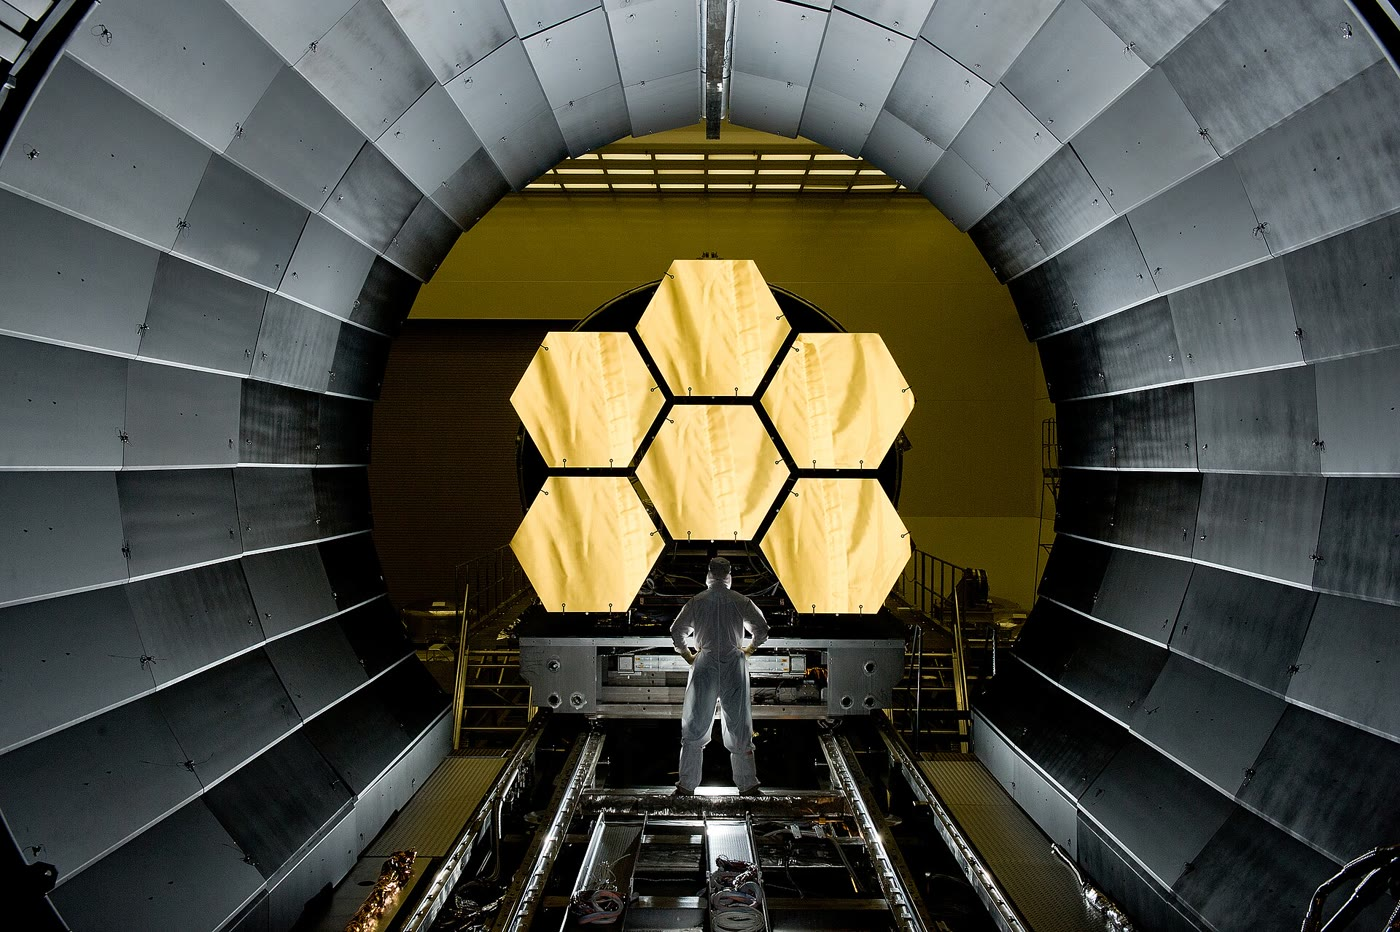
\includegraphics[width=0.78\linewidth]{images/book3/b1-jwst-mirror-segments.jpg}

{\small ست قطع من القطع السداسية الثماني عشرة للمرآة الرئيسية لتلسكوب جيمس ويب الفضائي، أُعدّت للاختبار البارد عام 2011؛ وحين تُفرد في الفضاء تكوّن القطع الثماني عشرة معًا مرآةً عرضها \qty{6.5}{m}. الصورة: NASA/MSFC/David Higginbotham، في الملك العام.}
% ledger: commons:jwst-mirror, nasa:jwst-mirror
\end{omfigure}

\section{التمارين}

\begin{exercise}[$\star$]\label{exo:b1:observing-the-sky:1}
ما نسبة دفقي نجمين قدراهما 1.0 و6.0؟ وما نسبة دفق ريجل ($V = 0.13$) إلى دفق بولاريس ($V = 2.02$)؟ أيّهما أسطع في السماء؟
\end{exercise}

\begin{exercise}[$\star$]\label{exo:b1:observing-the-sky:2}
اختلاف ألتير المنظري \ang{;;0.19495}. أعطِ بُعده \omterm{def:b1:observing-the-sky:parallax}{بالفرسخ الفلكي}، وبالوحدات الفلكية، وبالسنوات الضوئية.
\end{exercise}

\begin{exercise}[$\star$]\label{exo:b1:observing-the-sky:3}
احسب حدّ الحيود لتلسكوب فضائي قطره \qty{2.4}{m} عند \qty{550}{nm}، بالثواني القوسية، وقارنه برؤية فلكية قدرها \ang{;;0.40}. وافعل الشيء نفسه لتلسكوب قطره \qty{6.5}{m} عند \qty{2.0}{\micro\metre}.
\end{exercise}

\begin{exercise}[$\star$]\label{exo:b1:observing-the-sky:4}
رتّب من الجدول الخاص بالنجوم الأربعة الساطعة ريجل وألتير وبولاريس وبيتلجوز من السطح الأشدّ حرارةً إلى الأبرد. لماذا يمكن مقارنة \omterm{def:b1:observing-the-sky:colour-index}{دليل اللون} بين نجوم تبعد مسافات مختلفة كثيرًا؟
\end{exercise}

\begin{exercise}[$\star\star$]\label{exo:b1:observing-the-sky:5}
قيس نجم في الليلة نفسها، فكان قدره 6.412 عند بُعد زاوي عن \omterm{def:b1:spherical-astronomy:celestial-sphere}{سمت الرأس} قدره \ang{30}، وكان 6.590 عند \ang{60}. بافتراض غلاف جوي متوازي المستويات، احسب الكتلتين الهوائيتين، ومعامل الإخماد، وقدر النجم فوق الغلاف الجوي.
\end{exercise}

\begin{exercise}[$\star\star$]\label{exo:b1:observing-the-sky:6}
يعطي نجم 400 إلكترون ضوئي في تعريض مدته \qty{10}{s}، ويغلب ضجيج الفوتونات الصادر من النجم وحده. ما \omterm{def:b1:observing-the-sky:detector}{نسبة الإشارة إلى الضجيج}؟ وكم يجب أن يدوم التعريض لبلوغ نسبة 100؟ ولقياس القدر بدقة \num{0.01}؟
\end{exercise}

\begin{exercise}[$\star\star$]\label{exo:b1:observing-the-sky:7}
لريجل $V = 0.13$ واختلاف منظري قدره \ang{;;0.00378}. مع إهمال الإخماد بيننا وبينه، احسب بُعده وقدره المطلق وإشعاعيته في النطاق V بالوحدات الشمسية ($M_\odot = 4.83$).
\end{exercise}

\begin{exercise}[$\star\star$]\label{exo:b1:observing-the-sky:8}
قارن المساحتين المجمِّعتين لمرآة دائرية قطرها \qty{2.4}{m} (أهمل حجب مركزها) ولتلسكوب ويب (\qty{25}{m^2}). بكم يكون التعريض الذي يجمع فيه تلسكوب ويب العدد نفسه من الفوتونات أقصر؟ وما الكسر الذي تمثّله مساحته المجمِّعة من قرص كامل قطره \qty{6.5}{m}، ولماذا هو أقل من الواحد؟
\end{exercise}

\begin{exercise}[$\star\star$]\label{exo:b1:observing-the-sky:9}
(أ) انطلاقًا من \omterm{def:b1:observing-the-sky:flux}{إشعاعية} الشمس، \qty{3.828e26}{W}، احسب دفقها عند \qty{10}{\parsec}. (ب) القدران الظاهري والمطلق للشمس هما $-26.74$ و$4.83$. استعمل \omterm{def:b1:observing-the-sky:absolute}{معامل المسافة} لاستخراج بُعد الشمس عن الأرض، بالوحدات الفلكية.
\end{exercise}

\begin{exercise}[$\star\star\star$]\label{exo:b1:observing-the-sky:10}
بيّن انطلاقًا من \cref{prop:b1:observing-the-sky:bouguer} أن $k =
2.5\log_{10}e\;\tau_0$. وبالنسبة إلى ليلة خط الإخماد ($k =
\num{0.160}$)، احسب العمق البصري عند \omterm{def:b1:spherical-astronomy:celestial-sphere}{سمت الرأس} $\tau_0$، والكسر من الضوء الذي يبلغ التلسكوب عند \omterm{def:b1:spherical-astronomy:celestial-sphere}{سمت الرأس} وعند $X = 2.31$. ماذا يتنبأ به غلاف جوي متوازي المستويات للكتلة الهوائية عند بُعد زاوي عن \omterm{def:b1:spherical-astronomy:celestial-sphere}{سمت الرأس} قدره \ang{85}، ولماذا لا ينبغي الوثوق بهذه القيمة؟
\end{exercise}

\begin{exercise}[$\star\star\star$]\label{exo:b1:observing-the-sky:11}
تعطي مجرة خافتة $R = 50$ إلكترونًا ضوئيًا في الثانية في تلسكوب، وتعطي السماء في مساحة صورتها $B = \num{2000}$ في الثانية عندما تكون \omterm{def:b1:observing-the-sky:seeing}{الرؤية الفلكية} \ang{;;0.80}. ضجيج القراءة مهمل. (أ) كم يجب أن يدوم التعريض لنسبة إشارة إلى ضجيج قدرها 10؟ (ب) تنمو السماء في الصورة مع مساحة قرص \omterm{def:b1:observing-the-sky:seeing}{الرؤية الفلكية}. كرّر الحساب من أجل رؤية فلكية قدرها \ang{;;0.40}. (ج) بيّن أنه بالنسبة إلى مصدر أخفت بكثير من السماء، يتناسب زمن التعريض اللازم لنسبة إشارة إلى ضجيج معيّنة مع $\theta^2/D^2$، حيث $\theta$ \omterm{def:b1:observing-the-sky:seeing}{الرؤية الفلكية} و$D$ قطر التلسكوب.
\end{exercise}

\begin{exercise}[$\star\star\star$]\label{exo:b1:observing-the-sky:12}
محزوز فيه 1200 خط في المليمتر، مضاء على \qty{100}{mm}، ويُستعمل في الرتبة الأولى. (أ) ما قدرته على التفريق، وما أصغر فرق في الطول الموجي قابل للفصل عند \qty{550}{nm}؟ (ب) ما السرعة الشعاعية التي يقابلها هذا الفرق؟ (ج) تدور الأرض حول الشمس بسرعة \qty{29.78}{km.s^{-1}}. بكم يمكن لهذه الحركة أن تزيح خطًّا عند \qty{550}{nm}، وكم عنصر تفريق يمثّل ذلك؟ وماذا يجب أن يفعل الراصد الذي يقيس سرعة نجم إذن؟
% ledger: earth:vorb
\end{exercise}

\section{مسألة: وزن ضوء سيريوس}

\begin{problem}[{مسألة نهاية الأسبوع --- كم يبعد سيريوس، وكم يبدو ساطعًا، وكم فوتونًا يرسل، وكم شمسًا يفوق ضوؤه}]
\label{pb:b1:observing-the-sky:1}
% ledger: simbad:sirius, simbad:vega, simbad:sirius-b, nasa:sun-V, sun:Mabs, const:au
% numbers computed in the scratch calculator calc/ch02.py from the rounded data
لسيريوس، ألمع نجوم السماء الليلية، رفيق خافت هو القزم الأبيض سيريوس~B. استعمل المعطيات الآتية:
\begin{center}
\small
\begin{tabular}{lcc}
\hline
الجسم & $V$ & الاختلاف المنظري \\
\hline
سيريوس & $-1.46$ & \ang{;;0.37921} \\
سيريوس B & $8.44$ & --- \\
فيغا & $0.03$ & \ang{;;0.13023} \\
الشمس & $-26.74$ & --- \\
\hline
\end{tabular}
\end{center}
مع $M_\odot = 4.83$ في V، و$\qty{1}{\parsec} = \qty{206265}{\au} =
\qty{3.0857e16}{m} = \qty{3.2616}{\lightyear}$، ومعامل الإخماد $k = 0.15$ لكل كتلة هوائية عند المرصد.

\medskip
\noindent\textbf{الجزء الأول --- كم يبعد سيريوس؟}
\begin{enumerate}
  \item احسب بُعد سيريوس \omterm{def:b1:observing-the-sky:parallax}{بالفرسخ الفلكي}.
  \item عبّر عنه بالوحدات الفلكية وبالأمتار.
  \item عبّر عنه بالسنوات الضوئية. منذ متى غادر الضوء الذي نراه الليلة سيريوس؟
  \item على مدار السنة، بأيّ زاوية كلية يتأرجح اتجاه سيريوس من جانب إلى آخر؟ قارنها برؤية فلكية قدرها \ang{;;0.40}. لماذا يمكن قياس التأرجح مع ذلك بجزء صغير من \omterm{def:b1:observing-the-sky:seeing}{الرؤية الفلكية}؟
  \item لو كان الاختلاف المنظري خاطئًا بمقدار \ang{;;0.001}، فبأيّ كسر يكون البعد خاطئًا، وبكم سنة ضوئية؟
\end{enumerate}

\medskip
\noindent\textbf{الجزء الثاني --- كم يبدو ساطعًا؟}
\begin{enumerate}[resume]
  \item احسب نسبة دفقي سيريوس وفيغا في V.
  \item احسب نسبة دفقي الشمس وسيريوس.
  \item احسب نسبة دفقي سيريوس وسيريوس~B.
  \item من مرصد بارانال يعبر سيريوس خط الزوال على ارتفاع \ang{82.09} (\cref{ch:b1:spherical-astronomy}). احسب \omterm{def:b1:observing-the-sky:extinction}{الكتلة الهوائية}، والإخماد، والقدر المقيس في تلك اللحظة.
  \item كرّر الحساب عند ارتفاع \ang{30}. أيّ كسر من الضوء يضيع في الطريق؟
  \item لماذا تُضلّل الصيغة $X = \sec z$ راصدًا يقيس سيريوس بعد طلوعه مباشرةً؟
\end{enumerate}

\medskip
\noindent\textbf{الجزء الثالث --- عدّ الفوتونات.}
تسجّل آلة تصوير على تلسكوب قطره \qty{1}{m} $\num{3.0e4}$ إلكترونًا ضوئيًا في الثانية من نجم قدره $V = 10.0$، بعد تصحيحه من الإخماد. وتحمل كل بكسل كحدٍّ أقصى $\num{1.0e5}$ إلكترون (سعة البئر الممتلئة).
\begin{enumerate}[resume]
  \item كم إلكترونًا ضوئيًا في الثانية تسجّل آلة التصوير من سيريوس~B؟
  \item كم يدوم التعريض الذي يعطي سيريوس~B نسبة إشارة إلى ضجيج قدرها 1000، مع ضجيج الفوتونات الصادر من النجم وحده؟ وما الخطأ في قدره عندئذٍ؟
  \item كم إلكترونًا ضوئيًا في الثانية تسجّل آلة التصوير من سيريوس؟
  \item إذا سقط \qty{20}{\percent} من ضوء سيريوس في أسطع بكسل فيها، فكم يستغرق ذلك البكسل حتى يمتلئ؟
  \item على الصورة، تترك الأجنحة الخافتة لصورة سيريوس عند موضع سيريوس~B، $10^{-4}$ من ضوء سيريوس في كل بكسل، ويجمع أسطع بكسل لسيريوس~B \qty{20}{\percent} من ضوئه هو. قارن المعدلين في ذلك البكسل.
  \item ما أطول تعريض لا يشبّع ذلك البكسل؟ واحسب \omterm{def:b1:observing-the-sky:detector}{نسبة الإشارة إلى الضجيج} لسيريوس~B في ذلك البكسل في تعريض مدته \qty{0.5}{s}، مع احتساب ضجيج الفوتونات من المصدرين. هل يمكن رصد سيريوس~B، وما الذي يجعل ذلك صعبًا؟
\end{enumerate}

\medskip
\noindent\textbf{الجزء الرابع --- كم شمسًا؟}
\begin{enumerate}[resume]
  \item احسب \omterm{def:b1:observing-the-sky:absolute}{معامل المسافة} لسيريوس.
  \item استنتج \omterm{def:b1:observing-the-sky:absolute}{القدر المطلق} لسيريوس في V، بمنزلتين عشريتين.
  \item احسب بُعد فيغا وقدرها المطلق.
  \item أيّ من سيريوس وفيغا أكثر \omterm{def:b1:observing-the-sky:flux}{إشعاعية} في V بذاتها، وبأيّ عامل؟
  \item ما \omterm{def:b1:observing-the-sky:magnitude}{القدر الظاهري} للشمس إذا رُئيت من بُعد سيريوس؟ وإذا أخذنا 6.0 أخفت قدرٍ يُرى بالعين المجردة في ليلة مظلمة، فهل تكون مرئية؟
  \item حتى أيّ بُعد يبقى سيريوس مرئيًا بالعين المجردة؟
  \item احسب \omterm{def:b1:observing-the-sky:flux}{إشعاعية} سيريوس في النطاق V بالوحدات الشمسية: كم شمسًا يفوق سيريوس ضوءًا؟
\end{enumerate}
\end{problem}
